\section{DAPHNE Firmware}
\label{sec:firmware}

Each DAPHNE board has 8 AFE's for a total of 40 analog channels, the analog to digital conversion resolution is 14 bits,  and the sampling rate is 62.5MSPS. %The reading out of the expected data volume implies the use of dedicated firmware involving self-trigger scheme and zero suppression algorithms.  
A differential data bus is used in order to read all the digitized signals, the DDR data format can be seen in figure~\ref{fig:Datos_AFE}.

\begin{figure}
\centering % \begin{center}/\end{center} takes some additional vertical space
%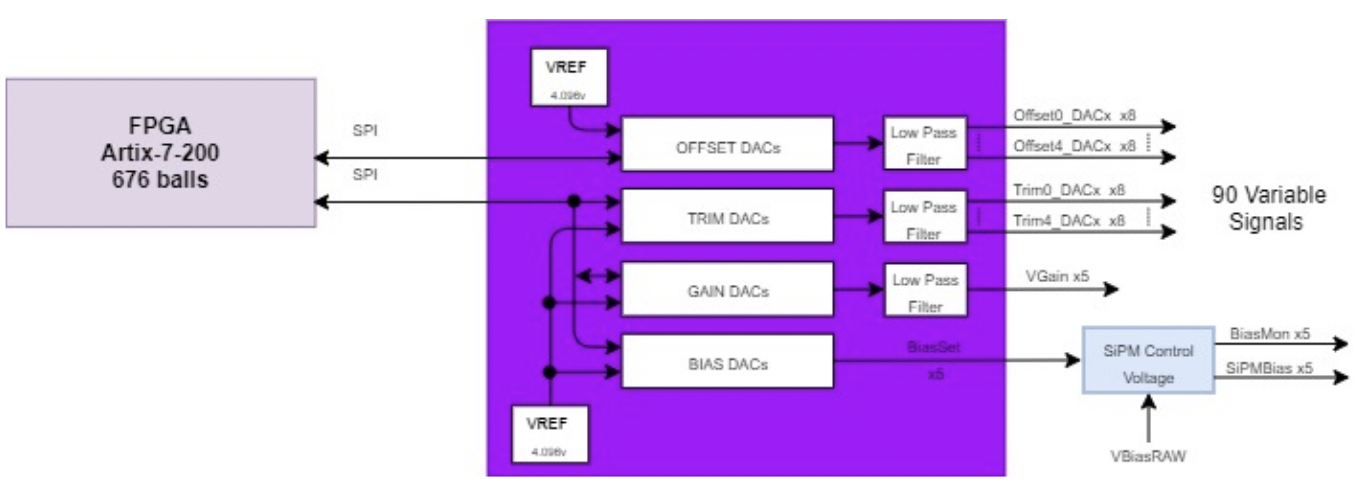
\includegraphics[width=.8\textwidth,trim=30 110 0 0,clip]{Images/BiasControl.png}
%\qquad
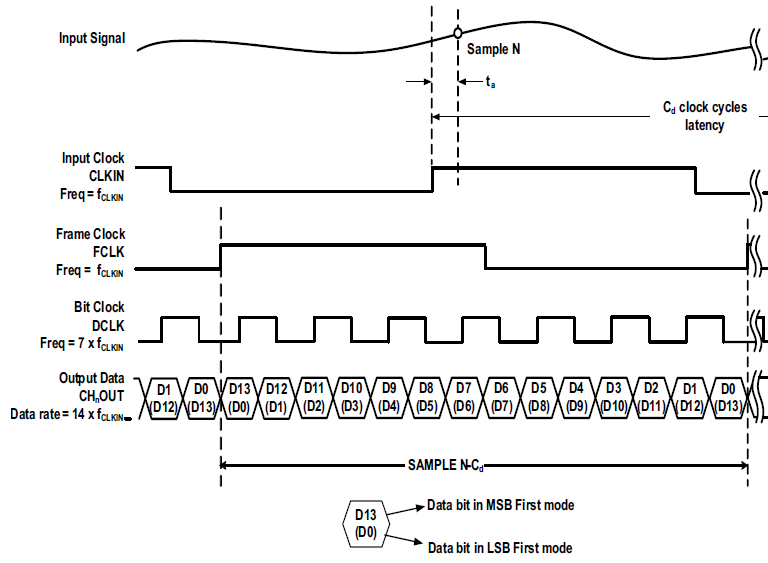
\includegraphics[scale=0.7,origin=c,angle=0]{Images/serial_data_AFE.png}
% "\includegraphics" from the "graphicx" permits to crop (trim+clip)
% and rotate (angle) and image (and much more)
\caption{\label{fig:Datos_AFE} Scheme of serial data reading on an AFE.}
\end{figure}

In order to have a proper DDR reading, the alignment of the digital clock with the center of the data bits is a must, and there are 2 common methods to do it. 

The first one, uses a PLL with multi-phase outputs. In this method, the FPGA uses the clock delivered by the AFE, pass it through a PLL primitive to align the phase of the data clock with the center of the data bits,  to finally obtain a simultaneous alignment of the 8 channels with the digital clock. 

In the second method, discrete time delays are applied to each data signal, these are added by a dedicated FPGA primitive called IDELAY. One should add as many delays are necessary to align each center of the data bit, with the digital clock that comes from the AFE.

Once the data bit is aligned with the bit clock, another process shall be made, in order to align the 14 bit frame with the frame clock. This process is named bitslip, and is an embedded functionality of the used HDL primitive called ISERDES.\cite{XILINX_Ref1:XAPP585,limitinganalog,semiconductor2009high}

At the moment of writing this paper both reading methods are implemented and a test of the performance of each is undergoing.


\subsection{Microcontroller Firmware}

The microcontroller performs the Slow Control, which is the interface of configuration and fitting of the different digitization parameters through the peripherals that carry out the conditioning, in addition to monitoring some variables of the DAPHNE board.

The microcontroller was configured to use Real Time Operating Systems (RTOS) to perform the activities proposed in the Slow Control. RTOS allows to efficiently distribute the tasks to be performed, redundantly evaluate the monitoring variables and avoid the microcontroller to inter in a halted state. The Figure \ref{fig:FirmwareMCU} shows the configuration scheme of the microcontroller.

\begin{figure}[htbp]
\centering % \begin{center}/\end{center} takes some additional vertical space
%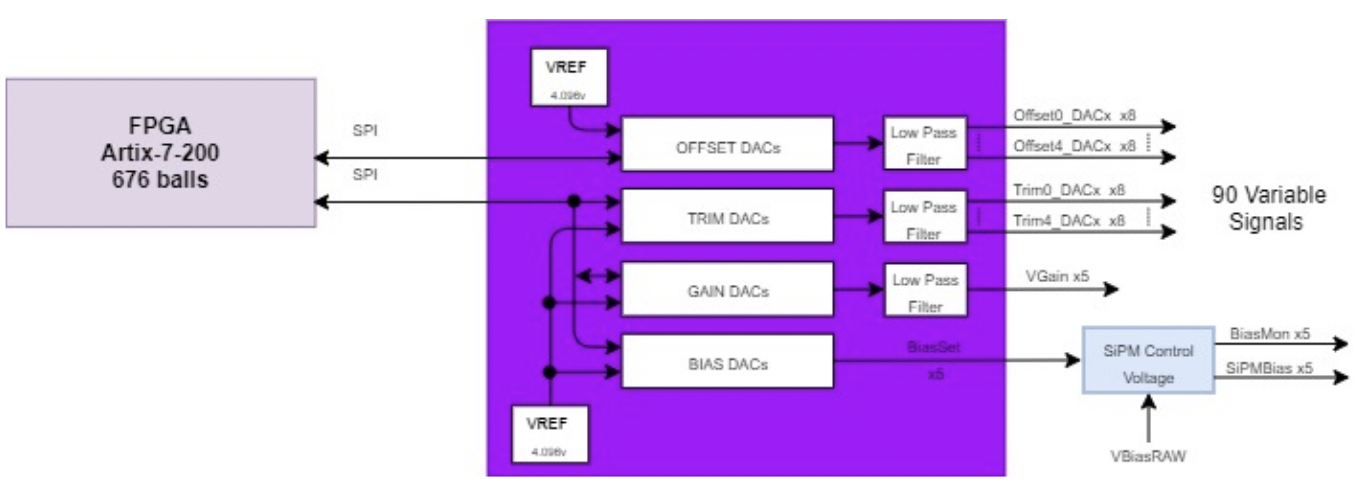
\includegraphics[width=.8\textwidth,trim=30 110 0 0,clip]{Images/BiasControl.png}
%\qquad
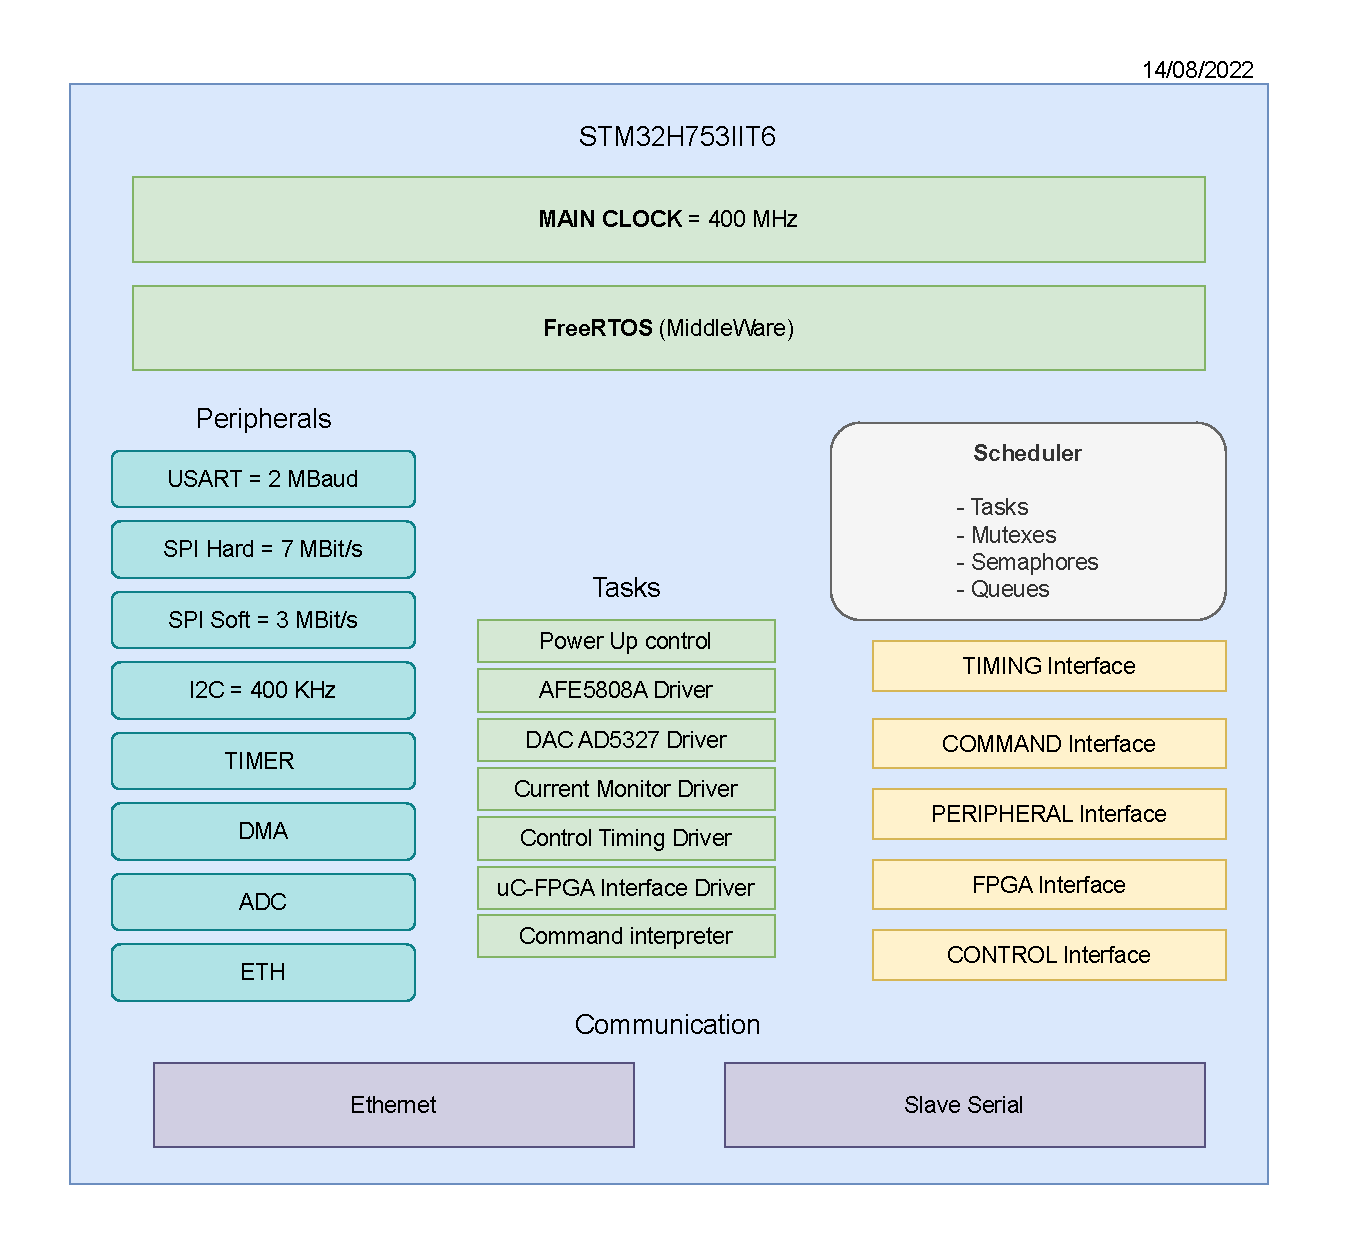
\includegraphics[width=0.8\textwidth,origin=c,angle=0]{Images/FirmwareMCU.pdf}
% "\includegraphics" from the "graphicx" permits to crop (trim+clip)
% and rotate (angle) and image (and much more)
\caption{\label{fig:FirmwareMCU} Microcontroller configuration scheme.}
\end{figure}

This diagram shows the configuration of the different peripherals of the microcontroller highlighted in aqua. In green, the distribution of tasks handled by the RTOS are highlighted. In yellow are presented the interfaces implemented to control and configure DAPHNE. Finally, the implemented communication interfaces highlighted in purple are presented.

This section describes the different stages that compose the firmware implemented in the microcontroller to perform the peripheral control, configuration and monitoring. 


\subsection{FreeRTOS (MiddleWare)}

FreeRTOS is a real-time operating system developed mainly for embedded devices, microcontrollers and small microprocessors. FreeRTOS has been adopted and implemented on more than 35 platforms including ARM and it is currently distributed under the MIT license. FreeRTOS implements methods for multiple threads, mutexes, semaphores, queues and software timers. It allows thread priority to be determined and device-specific interruptions to be handled. FreeRTOS also has a thread marking system that switches tasks according to their priority in a round-robin scheduling scheme \cite{freertos}. All these characteristics make it ideal for the implementation of highly complex and multitasking software such as that required in Slow Control for DAPHNE.


The firmware for DAPHNE was designed to perform six main tasks: Peripheral initialization, internal board monitoring, peripheral configuration and control, command interface, FPGA Bitstream load management, and Open Platform Communications Unified Architecture (OPC-UA) Server. Each of these tasks uses hardware and memory resources of the microcontroller that must be shared. Therefore this management with FreeRTOS allows the use of signaling through mutexes, semaphores, and its scheduler to handle the execution of the different tasks as multiple threads to avoid a possible collision.


\subsection{Peripheral initialization}

This task performs the initialization of all the peripherals to which the microcontroller has access and that must have a specific initialization sequence to guarantee the correct functioning of DAPHNE. Figure \ref{fig:InitPeriTask} shows the operating diagram for the initial configuration of the peripherals.

\begin{figure}[htbp]
\centering % \begin{center}/\end{center} takes some additional vertical space
%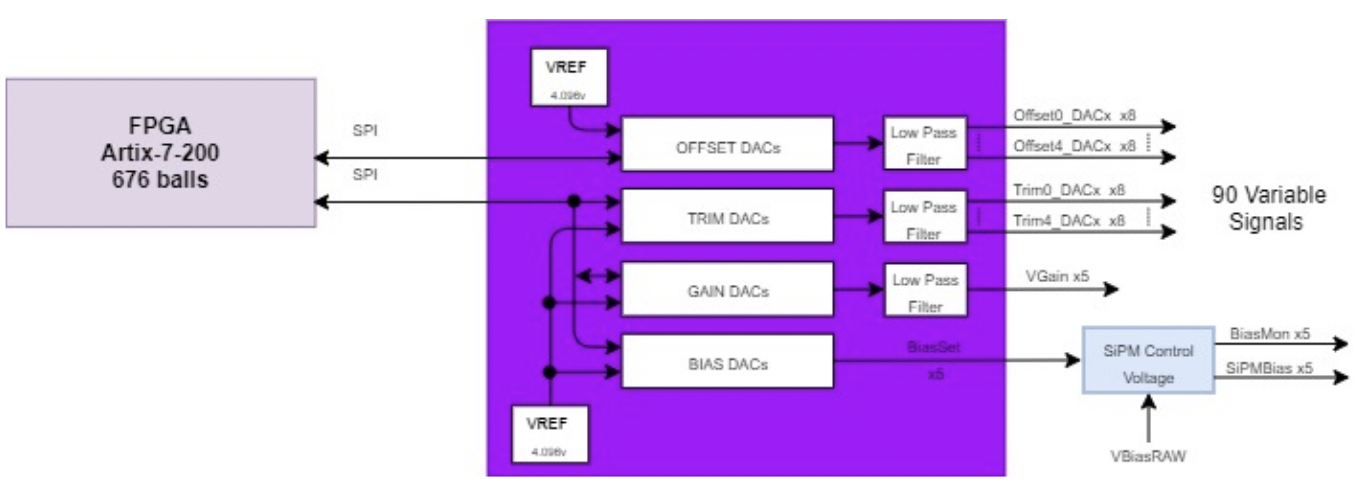
\includegraphics[width=.8\textwidth,trim=30 110 0 0,clip]{Images/BiasControl.png}
%\qquad
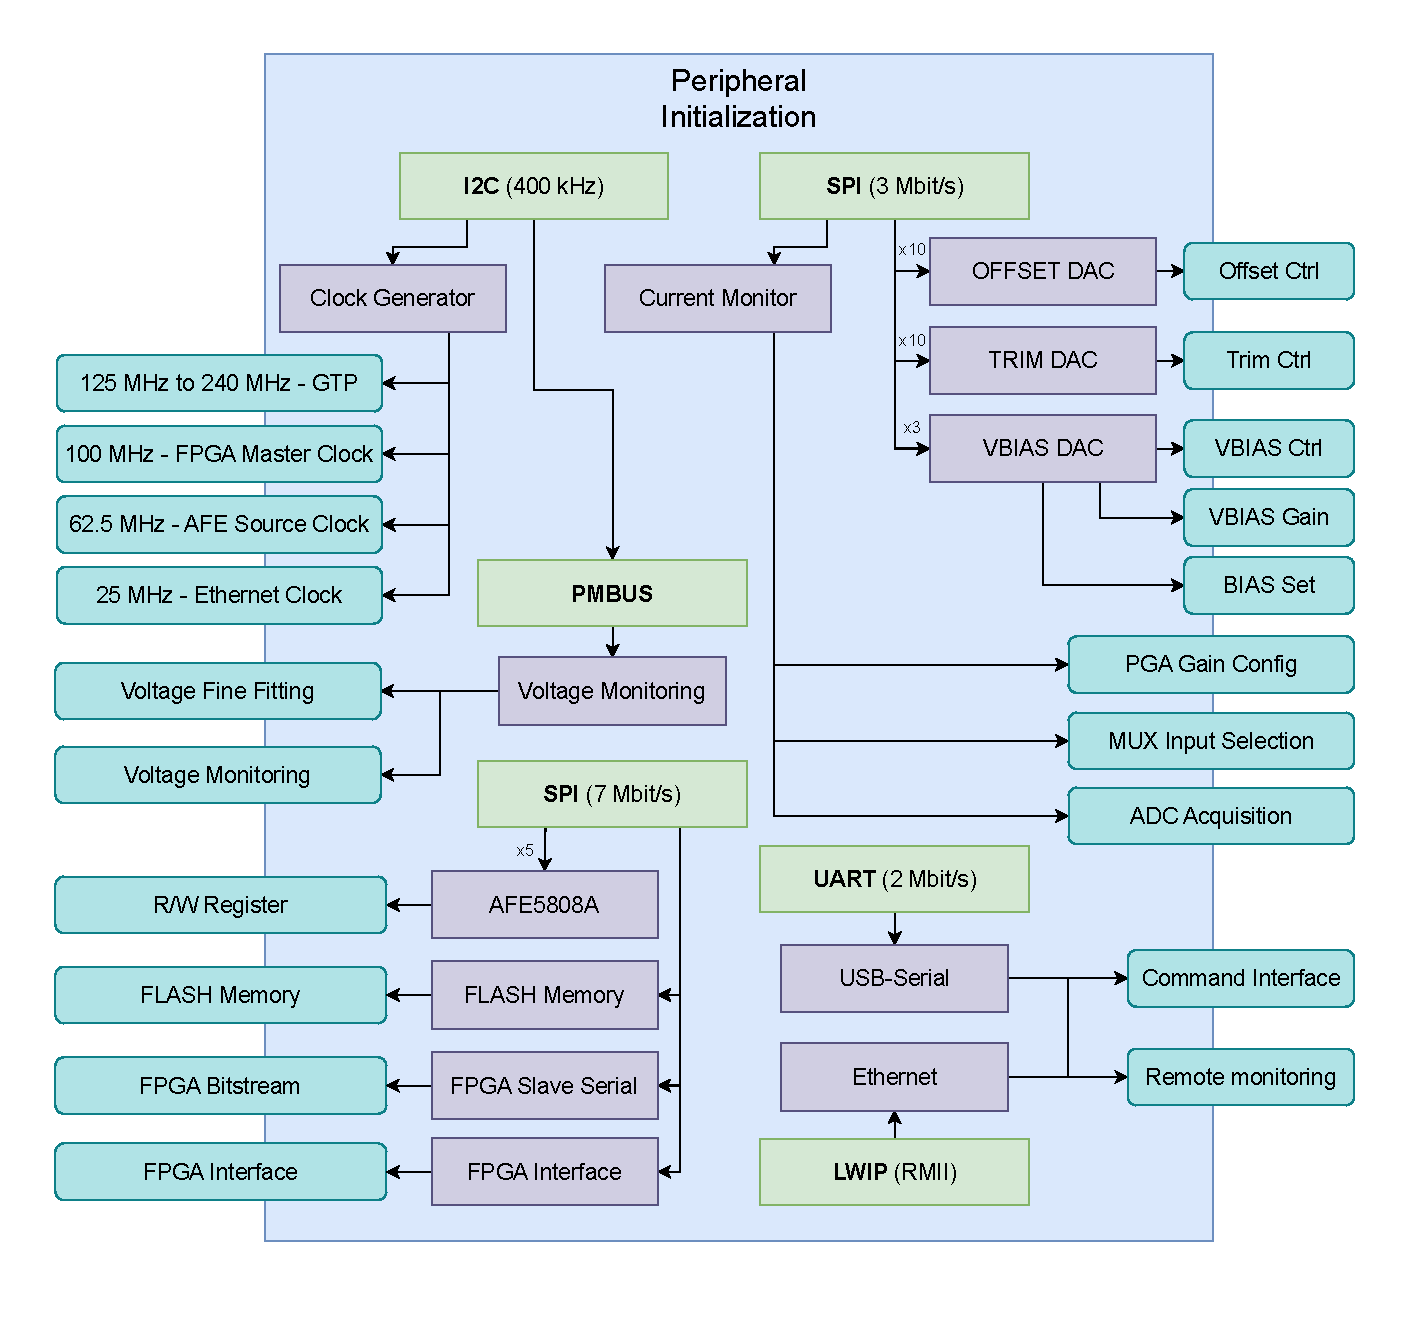
\includegraphics[width=0.9\textwidth,origin=c,angle=0]{Images/PeripheralInitTask.pdf}
% "\includegraphics" from the "graphicx" permits to crop (trim+clip)
% and rotate (angle) and image (and much more)
\caption{\label{fig:InitPeriTask} Peripheral initialization task scheme.}
\end{figure}

The first step in the configuration process is to configure the internal peripherals of the STM32H753IIT6 microcontroller \cite{stm32h7}. Once this configuration fits the requirements of each module, the initialization of the external peripherals is carried out through the writing of the internal memory registers to guarantee their operation in the desired mode.


\subsubsection{USART 2Mbit/s}

The Universal Serial Asynchronous Receiver Transmitter (USART) protocol was configured to be used at 2 Mbits/s with flow control by hardware. Also, the internal Interruption Service Routine (ISR) from the microcontroller was used to handle the data reception as events. All the information received through the USART module was handled by the Direct Memory Acces (DMA) module and stored in the FIFO structure of the RTOS Queue to prevent the collision in the use of memory resources of the microcontroller. The USART module aims to manage the Command Interface with a Host computer through a USB connection.


\subsubsection{SPI Hard 30Mbit/s 7Mbit/s and Soft 3Mbit/s}


One of the most useful features of the Serial Peripheral Interface (SPI) is the capability to connect multiple devices in the same communication bus. In this case, the microcontroller has six independent SPI modules which were used and distributed to the different peripherals. 

Two of them were used to control the AFE5808A at 7 Mbit/s to read and write the registers' memory and configure the different characteristics of these AFE modules. Also, to control the ADS5327BRUZ at 3 Mbit/s just to write the memory registers and control the voltage generated by each DAC in the subsystems (Trim DAC, Offset DAC, VBIAS DAC).

An SPI module was used to perform the Current Monitoring in the DAPHNE board, but also to control some AFE and DAC peripheral, sharing some hardware resources. This made it necessary to manage these resources through RTOS tasks separately. 

Also, an SPI module at 30 Mbit/s was used to control the FRAM and FLASH memory where some important configuration data is stored and the Bitstream for the FPGA respectively.

Finally, the other two SPI modules at 30 Mbit/s were used to implement a direct communication with the FPGA as a channel to configure or share some information between both processors and the other to load the Bitstream in the FPGA through the Slave Serial. 


\subsubsection{I2C 400kHz}

The Inter-Integrated Circuit (I2C) protocol allows connecting multiple devices in the same bus differentiated by their addresses. This module was configured with a 400 kHz clock signal to configure the Clock Generator and the PMBUS protocol to perform the Voltage Monitoring.

On the other hand, the PMBUS protocol allows to monitor the voltage generated by the voltage regulator and allows to fit the voltage value in a finer way.


\subsubsection{Ethernet}

The LwIP stack was used to configure the Ethernet module on the STM32H753IIT6 microcontroller. RMII was used as the peripheral configuration since it uses a reduced number of pins. High speed response was selected as the speed for the switching state of the pins associated with the Ethernet module.

As an important step in the configuration, it was necessary to enable the Memory Protection Unit (MPU) for the ICache and the DCache. Also, direct access to the microcontroller's D2RAM memory was defined. The PHY chip used in DAPHNE is the DP83620 which is a base 100 Mbit/s fiber optic transceiver \cite{dp83620}. The PHY receives the clock signal from the Clock Generator at 25 MHz.

The Ethernet was configured so that each DAPHNE had a unique MAC Address and a unique static IP, which can be configured from the command interface and is loaded from the FLASH memory when DAPHNE is started up.

In the application layer, the OPC-UA protocol was implemented in server mode to monitor some important variables of the board and to receive the commands that are then processed by the command interface.



\subsection{Board Monitoring}


The second task of the FreeRTOS is in charge of monitor peripheral functioning. This task executes the voltage monitoring, the current monitoring, and the Clocks Generation.

As was shown in Figure \ref{fig:InitPeriTask}, the voltage monitoring provides information about the state of the voltage power supply and the Bias and Trim voltage to inform the system about a possible risk of High power consumption that can affect the results of the experiment or damage the DAPHNE board, also with the current monitoring.

On the other hand, the Clock Generator produce four different clock signals:
 \begin{enumerate}
     \item GTP clock from 125 MHz to 240 MHz: This clock is configured by software through the command interface and is used to feed the GTP module.
     
     \item FPGA master clock at 100 MHz: This clock signal works as the master clock for the FPGA.
     
     \item AFEs source clock at 62.5 MHz: This clock is generated as a differential signal and it is directed to the FPGA where it is buffered to the clock fanout and distributed to the five AFEs separately.
     
     \item Ethernet clock at 25 MHz: This clock is used to feed the PHY chip.
     
 \end{enumerate}
 
Some of these clocks need to be synchronized to execute specific tasks like the alignment of the AFE's readout data and the Ethernet data transmission.


\subsection{Peripheral Configuration and Control}



\begin{figure}[htbp]
\centering % \begin{center}/\end{center} takes some additional vertical space
%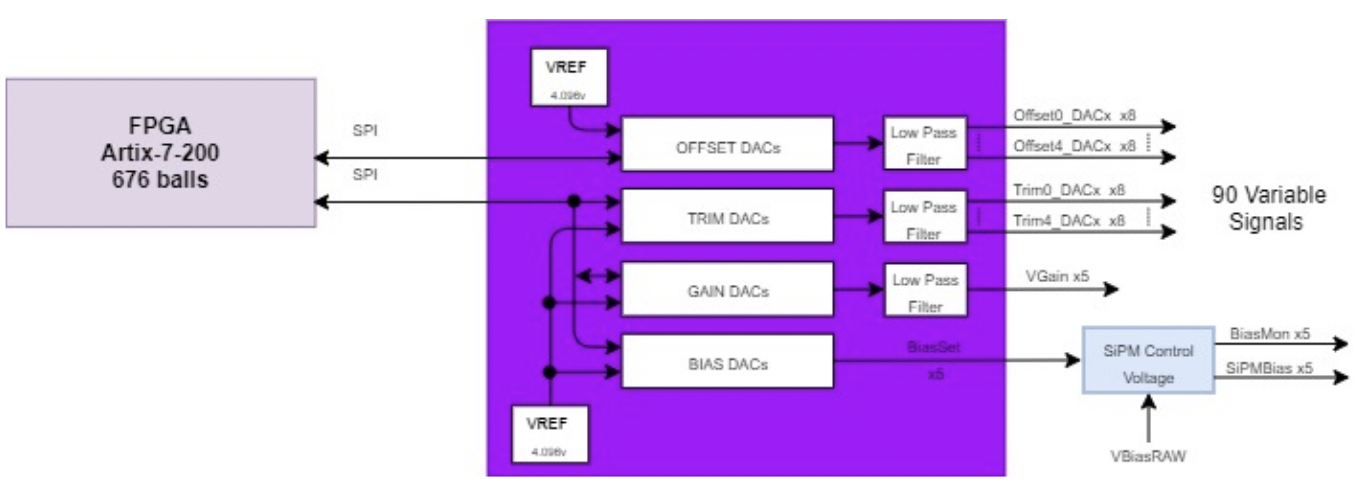
\includegraphics[width=.8\textwidth,trim=30 110 0 0,clip]{Images/BiasControl.png}
%\qquad
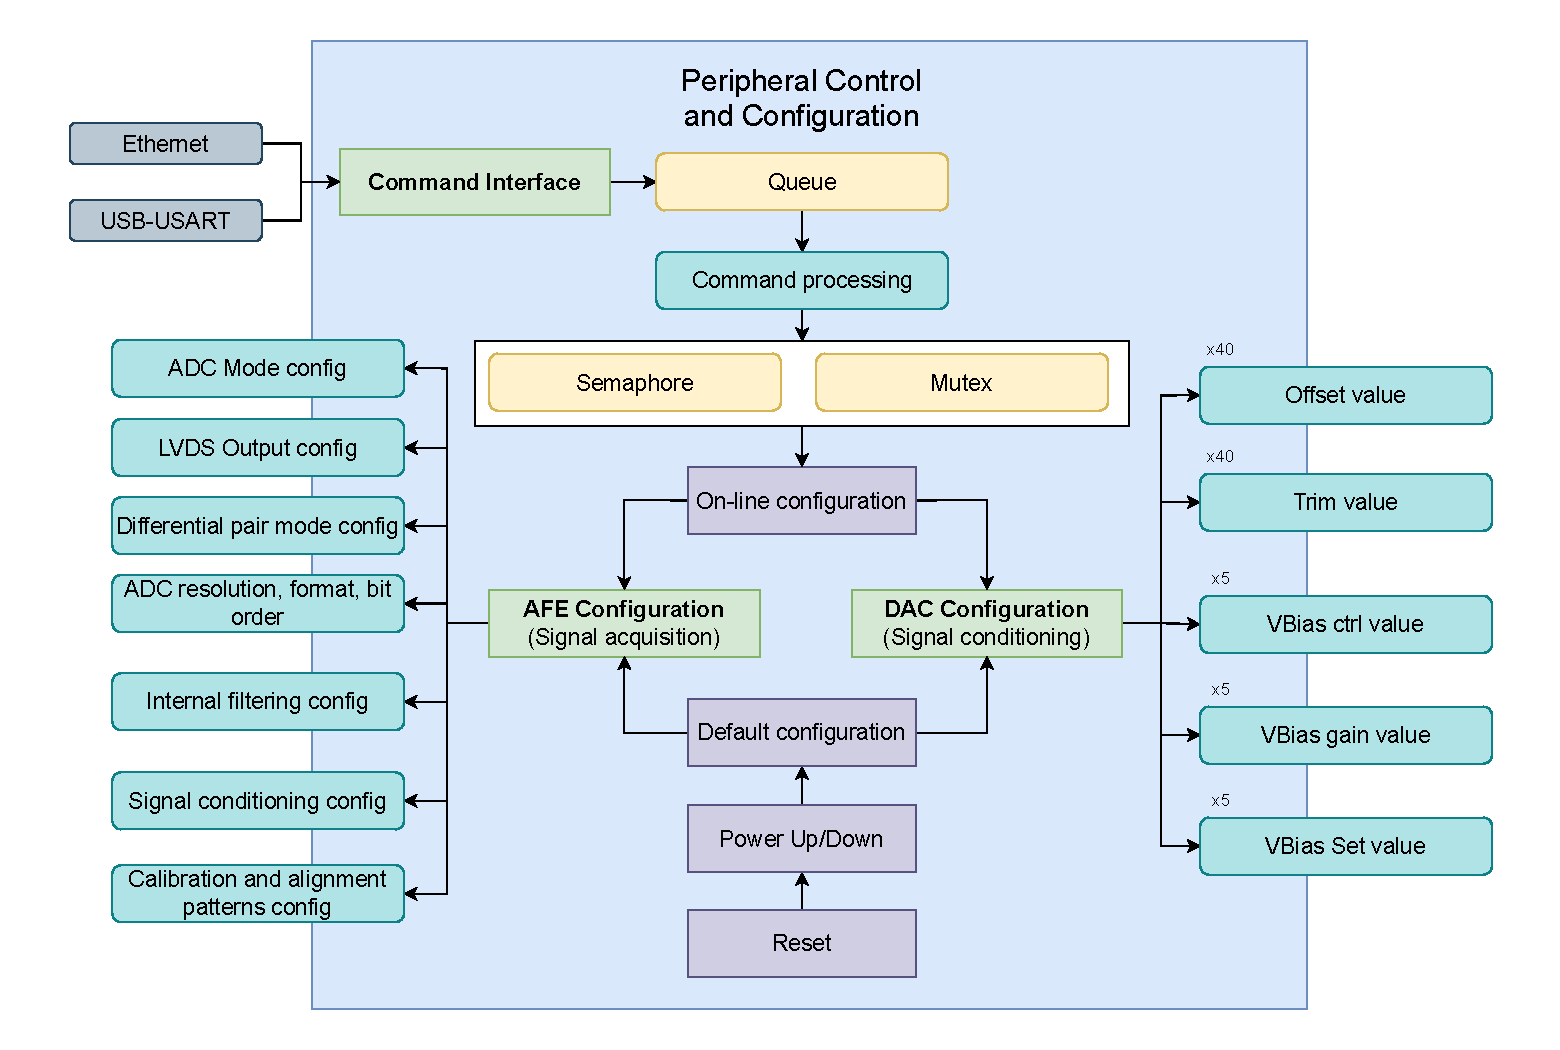
\includegraphics[width=0.9\textwidth,origin=c,angle=0]{Images/ControlTask.pdf}
% "\includegraphics" from the "graphicx" permits to crop (trim+clip)
% and rotate (angle) and image (and much more)
\caption{\label{fig:InitPeriTask} Control and configuration task scheme.}
\end{figure}





%Control de los diferentes perifericos para cambiar su configuracion en tiempo de ejecucion, esta tarea esta ligada con el command interface, y depende de la liberacion de recursos como QUEUEs, MUTEX, SEMAPHORES, 

%\subsubsection{Power Up control}

%Ajuste fino de los voltajes de los reguladores

%\subsubsection{AFE Configuration}

%COnfiguracion completa de los registros del AFE, tambien permite realizar la consulta de la configuracion actual 

%\subsubsection{DAC Driver}

%COnfiguracion y ajuste de los voltajes de salida de los DACs

%\subsubsection{Control Timing Driver}

%Control de los CLOCKs generados por el CDR

%\subsubsection{Current Monitor}

%Configuracion de las ganancias de los PGA, multiplexacion de las entradas para el monitoreo.



%\subsection{Command Interface}

%Interface de comandos que recibe los comandos para la ejecucion de difernetes acciones dentro del microcontrolador, los comandos pueden venir desde el USART o desde el OPC-UA a traves de ETH. los comandos son interpretados, gestioandos y direccionados principamnete a la tarea de configuracion y control de perifericos para ejecutar las acciones requeridas, una vez estas se han ejecutado, la interface de usuario envia una respuesta indicando el estado de la ejecucion.

%\subsubsection{Command interpreter}

%Explicar la estructura del command interpreter, y del command interface



%\subsection{FPGA Bitstream Load}

%Esta tarea se encarga de la comunicacion con la FPGA y con la memoria FRAM, almacenamiento del Bitstream, carga a la FPGA a alta velocidad a traves del Slave Serial, ademas de realizar streaming de datos a traves de una interface SPI hacia el microcontrolador de los datos recolectados a gran velocidad por los AFEs, datos previamente alineados en la FPGA

%\subsubsection{uC-FPGA Interface}

%Cpnexion SPI para gestion de comunicacion entre microcontrolador y FPGA

%\subsubsection{FRAM interface}

%Comuinicacion con la FRAM para almacenamiento y lectura del Bitstream de la FPGA

%\subsubsection{Slave Serial}

%Protocolo de envio del Bitstream hacia la FPGA, se implementa tambien un protocolo CRC para la verificacion de los datos enviados en el Bitstream




%\subsection{OPC-UA Server}

%Servidor OPC-UA para el monitoreo del estado de la tarjeta, consulta de las variables internas de DAPHNE, envio de comandos y recepcion de respuestas, todo gestionado a traves de este protocolo para acceder de manera remota y a traves de Ethernet a las diferentes tarjetas DAPHNE que componen el experimento de photodeteccion.

%\subsubsection{OPCUA}

%el OPC-UA permite gestionar la comunicaion con las diferentes tarjetas mediante las direcciones unicas que estas reciben por el protocolo Ethernet












